\documentclass[a4paper,10pt]{jsarticle}
% 数式
\usepackage{amsmath,amsfonts}
\usepackage{bm}
% 画像
\usepackage[dvipdfmx]{graphicx}
\usepackage[version=4]{mhchem}
\usepackage{here} %画像の表示位置調整用


%A4: 21.0 x 29.7cm


\begin{document}
  \section{有限温度のBCS理論の導出の概要}
  grand canonical分布を用いて平衡状態を考える。(温度$T$,化学ポテンシャル$\mu$はConst.)
  
  グランドポテンシャル$\Omega=E- TS -\mu N$から変分法を用いて
  密度op.$D$を定義し、$\operatorname{Tr}D=1$という性質で、これを用いれば分配関数と密度演算子
  は以下のように決められる。
  \begin{align}
    D &= Z^{-1}e^{-\beta(H-\mu N)}\\
    Z &= \operatorname{Tr}\left[e^{-\beta(H-\mu N)}\right]
  \end{align}
  また演算子$O$の期待値は、
  \begin{equation}
    \left\langle O\right\rangle=\operatorname{Tr}DO\label{期待値}
  \end{equation}
  である。
  これがHFB近似のもとではquasi-particle Hamiltonian\ $\operatorname{H_{\text{HFB}}}$が
  quasi-particle 真空エネルギー$E_0$,quasi-particle エネルギー$E_i$,
  quasi-particle creation op.$a_i^{\dagger}$を使って
  $\operatorname{H_{\text{HFB}}}=E_0 + \sum_{i}E_i a_i^{\dagger}a_i$
  と表すことができることから、HFB 密度演算子とHFB分配関数は
  \begin{align}
    D_{\text{HFB}} &= Z_{\text{HFB}}^{-1}\exp\left(-\beta \sum_i E_i \hat{n}_i\right)\\
    Z_{\text{HFB}} &= \operatorname{Tr}\left[\exp\left(-\beta \sum_i E_i \hat{n}_i\right)\right]
  \end{align}
  ただし、$\hat{n}_i = a_i^{\dagger}a_i$。
  この分配関数を展開すれば、
  \begin{align}
    Z_{\text{HFB}} &= \operatorname{Tr}\left[\exp\left(-\beta \sum_i E_i \hat{n}_i\right)\right]\\
    &= \sum_{n_i}\prod _{i} e^{-\beta E_i n_i}
  \end{align}
  となるが、quasi-particle近似において$n_i=0,1$であるから、$\hat{n}_i^2=\hat{n}_i$より、
  \begin{equation}
    Z=\prod _{i} \left(1 + e^{-\beta E_i}\right)
  \end{equation}
  と展開できる。
  これを使えば密度演算子は
  \begin{equation}
    D_{\text{HFB}} = Z_{\text{HFB}}^{-1}\prod _{i}
    \left[e^{-\beta E_i}\hat{n}_i + (1 - \hat{n}_i)\right]
  \end{equation}
  となる。ここは$n_i=0,1$を主に用いた。Fermi分布関数$f_i=1/(1 + e^{\beta E_i})$を使えば、
  \begin{equation}
    D_{\text{HFB}}=\prod_i \left[f_i\hat{n}_i+(1 - f_i)(1 - \hat{n}_i)\right]
  \end{equation}
  ここまではquasi-particleを使っていたので変換式
  $a_i^{\dagger} = \sum_{j}(U_{ij}c_j^{\dagger}+V_{ij}c_j)$から
  逆変換を行うことで単粒子の場合の密度とペアリングテンソルを求める。
  式(\ref{期待値})からそれぞれ、
  \begin{align}
    \rho_{ij} &= \langle c_j^\dagger c_i\rangle=\operatorname{Tr}D c_j^\dagger c_i\\
    t_{ij}    &= \left\langle c_j c_i\right\rangle=\operatorname{Tr}D c_j c_i
  \end{align}

  これを逆変換を行いながら
  $\bar{\rho}_{ij}=\langle a_j^\dagger a_i\rangle=\operatorname{Tr}D a_j^\dagger a_i=\delta_{ij}f_i,
  \bar{t}_{ij}=\langle a_j a_i\rangle=0$を用いて計算を進めると、
  \begin{align}
    \rho &= \tilde{U}fU^{*} + V^{\dagger}(1-f)V \\
    t    &= \tilde{U}fV^{*} + V^{\dagger}(1-f)U
  \end{align}
  のようになる。
  これは$T=0$のときに$f=0$になることから普段のBCS方程式と一致することがわかる。
  また、このときの粒子、空孔状態のエントロピー$S$と粒子数$N$は
  \begin{align}
    S &= -k\sum_{i}\left[f_i\ln f_i + (1-f_i)\ln (1 - f_i)\right]\\
    N &= \operatorname{Tr}\rho
  \end{align}
  その他の手続きは$T=0$のときとあまり変わらずに、Hamiltonianが、
  \begin{equation}
    H=\sum_{i}\epsilon_ic_i^{\dagger}c_i-\sum_{ij>0}G_{ij}c_i^{\dagger}c_{\bar{i}}^{\dagger}c_{\bar{j}}c_i
  \end{equation}
  としたときに、$E_i=E_{\bar{i}}=[(\epsilon_i -\mu)^2 +\Delta_i]^{1/2}$を用いて、
  \begin{align}
    u_i^2 = \dfrac{1}{2}(1+\epsilon_i/E_i)\\
    v_i^2 = \dfrac{1}{2}(1-\epsilon_i/E_i)
  \end{align}
  これを$U,V$に代入してペアリングテンソルを計算すれば、
  \begin{align}
    t_{i\bar{i}}=u_iv_i(1-2f_i)\\
    u_iv_i=-\dfrac{\Delta_i}{2E_i}\\
    1-2f_i=\tanh(1/2\beta E_i)
  \end{align}
  よってgap方程式は$\Delta_i=-\sum_{k>0}G_{ik}t_{k\bar{k}}$より、
  \begin{equation}
    \Delta = \dfrac{1}{2}\sum_{j>0}G\dfrac{\Delta}{E_j} \tanh{(1/2\beta E_j)}
  \end{equation}
  これは$T=0$のときに$\tanh = 1$となり一致する。
  \ce{{}^{116}Sn}の時の計算結果と温度は別紙に示す。
  
  研究名は
  有限温度下における\ce{Sn}核の超流動相転移解析:Woods-Saxonポテンシャルとシニオリティペアリングモデルの応用
  \begin{figure}[H]
    \centering
    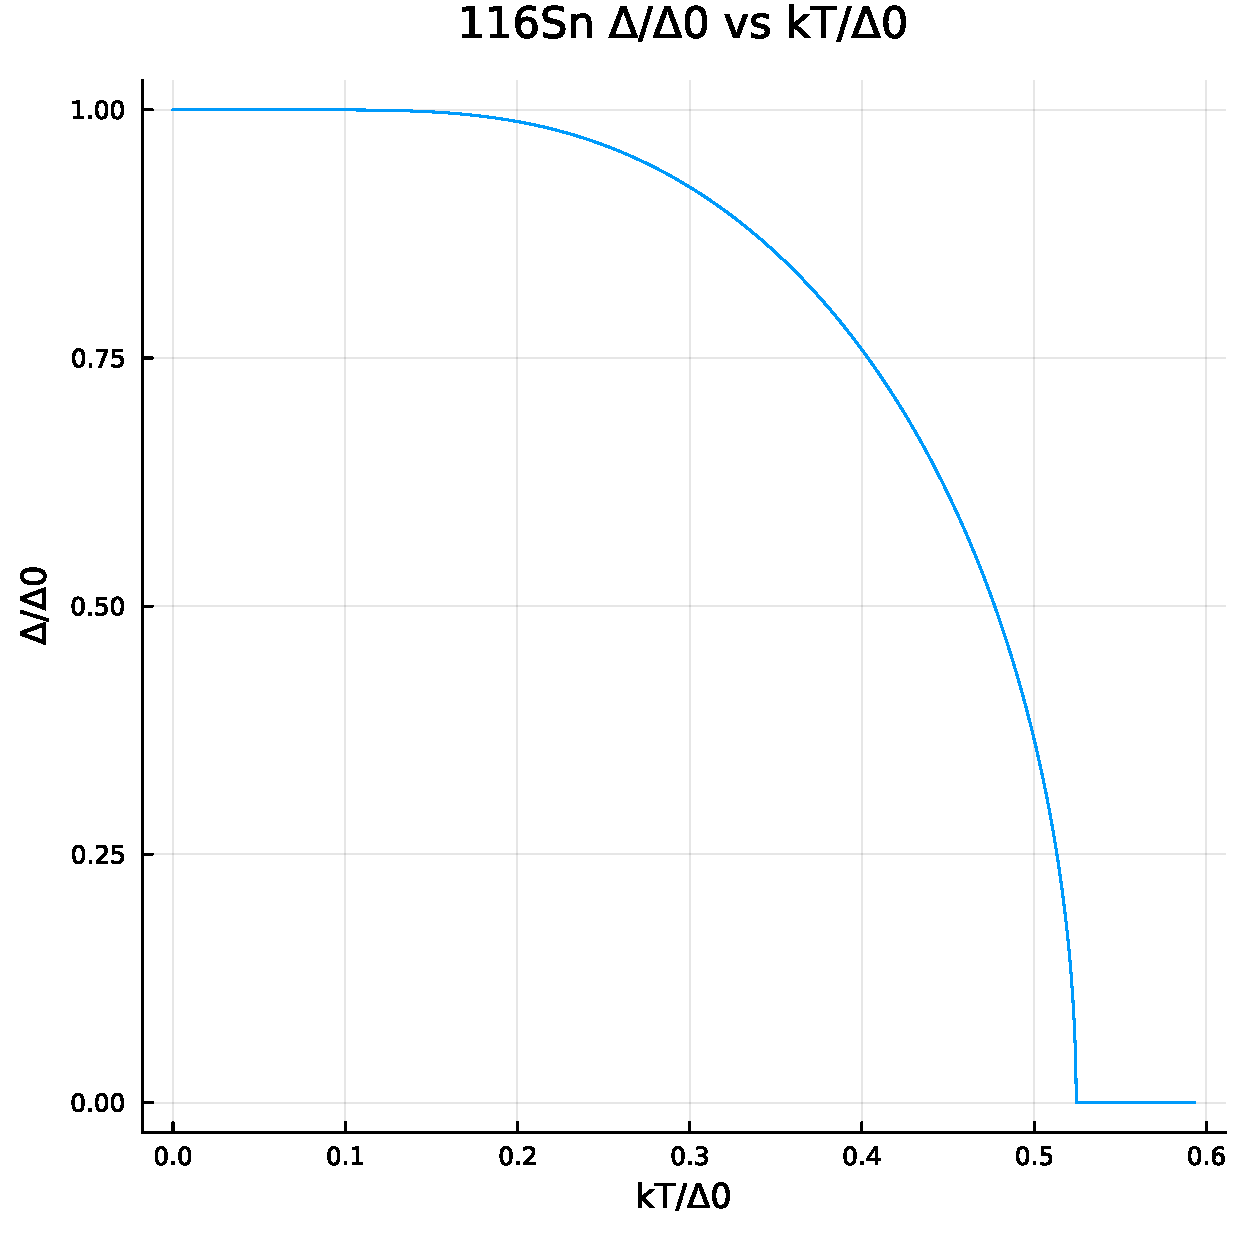
\includegraphics[width=0.8\textwidth]{02061.pdf}
    \caption{Pairing gap versus temperature in \ce{{}^{116}Sn}.$G=0.116,\lambda=-9.519$MeV}
  \end{figure}
  $kT\simeq0.6623$[MeV]より$T\simeq7.69\times 10^9$[K]

\end{document}